\subsection{Critical Error Detection}
\label{subsec:rootcause}

\noindent{\textbf{Dataset.}}
We evaluate critical error localization on \Bench{} (Sec.~\ref{sub:bench}), which consists of 200 annotated failure trajectories.  
These trajectories are drawn from three representative benchmarks: \textbf{ALFWorld} \citep{shridhar2020alfworld}, \textbf{GAIA} \citep{mialon2023gaia}, and \textbf{WebShop} \citep{yao2022webshop}.  

\noindent{\textbf{Baselines.}}
We compare against three strategies: (1) \textbf{Direct Prompting}, which queries the LLM directly for error localization without any structured search; (2) \textbf{Brute Force}, which examines steps sequentially from $t{=}1$ to $T$, substituting a corrected action at each step and stopping once the rollout succeeds, thereby identifying the earliest critical step; and (3) \textbf{Binary Search}, which applies a divide-and-conquer procedure by probing the midpoint of the trajectory and recursively halving the search space until the critical step is isolated.  

\noindent{\textbf{Implementation.}}
We use GPT-4.1 as the base model, with the temperature set to 0 for deterministic outputs. The full prompt template is provided in the Appendix \ref{app:prompt}. 

\noindent{\textbf{Evaluation Metic.}} We evaluate critical error detection at multiple granularities, capturing both partial and complete localization ability. Specifically, we measure \textbf{Step} accuracy, the ability to identify the exact step where the first critical error occurs; %\textbf{Error Type} accuracy, the assignment of the correct fine-grained \AET{} label (e.g., constraint ignorance, format error); 
\textbf{Step+Module} accuracy, the joint prediction of both the correct step and its module; and \textbf{All Correct} (Step+Module+Error Type), a strict metric requiring the exact step, module, and error type to all be correctly identified.


\noindent{\textbf{Experiment Results}}  
Table~\ref{tab:exp1} shows that \ModelName{} consistently surpasses baselines across datasets and metrics. On average, \ModelName{} is 24\% more accurate in the All-Correct metric (24.3\% vs.\ 0.3\%) and improves Step accuracy by 61\% (45.0\% vs.\ 28.0\%). The gains are especially pronounced on GAIA, where Step accuracy nearly doubles (58.0\% vs.\ 30.0\%) and All-Correct triples (38.0\% vs.\ 12.0\%).

\begin{table}[hbtp]
\centering
\definecolor{GreenDark}{HTML}{34A853}
\definecolor{GreenLight}{HTML}{E6F4EA}
% 2. WebShop - 橙色系
\definecolor{OrangeDark}{HTML}{FBBC04}
\definecolor{OrangeLight}{HTML}{FEF8E7}
% 3. GAIA - 紫色系
\definecolor{PurpleDark}{HTML}{A142F4}
\definecolor{PurpleLight}{HTML}{F3E8FD}
% 4. Average - 粉色系
\definecolor{PinkDark}{HTML}{FF6D70}
\definecolor{PinkLight}{HTML}{FFEEEE}

\setlength{\tabcolsep}{6pt} % 调整列间距
\renewcommand{\arraystretch}{1.2} % 调整行高

\resizebox{\linewidth}{!}{\begin{tabular}{l ccc ccc ccc ccc}
\toprule
& \multicolumn{3}{c}{\cellcolor{GreenDark}\color{white}\textbf{ALFWorld}}
& \multicolumn{3}{c}{\cellcolor{OrangeDark}\color{white}\textbf{WebShop}}
& \multicolumn{3}{c}{\cellcolor{PurpleDark}\color{white}\textbf{GAIA}}
& \multicolumn{3}{c}{\cellcolor{PinkDark}\color{white}\textbf{Average}} \\

\cmidrule(lr){2-4} \cmidrule(lr){5-7} \cmidrule(lr){8-10} \cmidrule(lr){11-13}

% --- 表头第二行：S, S+M, ALL ---
\textbf{Method}
& \cellcolor{GreenDark}\color{white}S & \cellcolor{GreenDark}\color{white}S+M & \cellcolor{GreenDark}\color{white}ALL
& \cellcolor{OrangeDark}\color{white}S & \cellcolor{OrangeDark}\color{white}S+M & \cellcolor{OrangeDark}\color{white}ALL
& \cellcolor{PurpleDark}\color{white}S & \cellcolor{PurpleDark}\color{white}S+M & \cellcolor{PurpleDark}\color{white}ALL
& \cellcolor{PinkDark}\color{white}S & \cellcolor{PinkDark}\color{white}S+M & \cellcolor{PinkDark}\color{white}ALL \\
\midrule

% --- 数据行：Baseline 方法 ---
Direct Prompting
& \cellcolor{GreenLight}28.0\% & \cellcolor{GreenLight}14.0\% & \cellcolor{GreenLight}1.0\%
& \cellcolor{OrangeLight}30.0\% & \cellcolor{OrangeLight}6.0\% & \cellcolor{OrangeLight}0.0\%
& \cellcolor{PurpleLight}26.0\% & \cellcolor{PurpleLight}10.0\% & \cellcolor{PurpleLight}0.0\%
& \cellcolor{PinkLight}28.0\% & \cellcolor{PinkLight}10.0\% & \cellcolor{PinkLight}0.3\% \\

Brute Force
& \cellcolor{GreenLight}10.0\% & \cellcolor{GreenLight}5.0\% & \cellcolor{GreenLight}0.0\%
& \cellcolor{OrangeLight}8.0\% & \cellcolor{OrangeLight}0.0\% & \cellcolor{OrangeLight}0.0\%
& \cellcolor{PurpleLight}18.0\% & \cellcolor{PurpleLight}8.0\% & \cellcolor{PurpleLight}0.0\%
& \cellcolor{PinkLight}12.0\% & \cellcolor{PinkLight}4.3\% & \cellcolor{PinkLight}0.0\% \\

Binary Search
& \cellcolor{GreenLight}20.0\% & \cellcolor{GreenLight}6.0\% & \cellcolor{GreenLight}1.0\%
& \cellcolor{OrangeLight}14.0\% & \cellcolor{OrangeLight}8.0\% & \cellcolor{OrangeLight}0.0\%
& \cellcolor{PurpleLight}22.0\% & \cellcolor{PurpleLight}10.0\% & \cellcolor{PurpleLight}0.0\%
& \cellcolor{PinkLight}18.7\% & \cellcolor{PinkLight}8.0\% & \cellcolor{PinkLight}0.3\% \\
\midrule

\textbf{\ModelName{}}
& \cellcolor{GreenLight}\textbf{35.0\%} & \cellcolor{GreenLight}\textbf{28.0\%} & \cellcolor{GreenLight}\textbf{21.0\%}
& \cellcolor{OrangeLight}\textbf{42.0\%} & \cellcolor{OrangeLight}\textbf{22.0\%} & \cellcolor{OrangeLight}\textbf{14.0\%}
& \cellcolor{PurpleLight}\textbf{58.0\%} & \cellcolor{PurpleLight}\textbf{44.0\%} & \cellcolor{PurpleLight}\textbf{38.0\%}
& \cellcolor{PinkLight}\textbf{45.0\%} & \cellcolor{PinkLight}\textbf{31.3\%} & \cellcolor{PinkLight}\textbf{24.3\%} \\

\bottomrule
\end{tabular}}
\caption{Comparison of methods across three environments (ALFWorld, WebShop, GAIA) and their average performance. Our method consistently outperforms baselines in all settings. Metrics shown are Step Exact (S), Step+Module (S+M), and All Correct (ALL).}
\label{tab:exp1}
\end{table}




% \begin{table}[htbp]
% \centering
% \small
% \renewcommand{\arraystretch}{1.0} % Adjust row spacing
% \setlength{\tabcolsep}{6pt} % Adjust column spacing
% \resizebox{\linewidth}{!}{
% \begin{tabular}{
%     l
%     |>{\columncolor{Color1}}c
%     |>{\columncolor{Color2}}c
%     |>{\columncolor{Color3}}c
%     |>{\columncolor{Color4}}c
%     |>{\columncolor{Color5}}c
%     |>{\columncolor{Color6}}c
% }
% \toprule
% \textbf{Method} & \textbf{Step} & \textbf{Step ($\pm$3)} & \textbf{Module} & \textbf{Error Type} & \textbf{Step+Module} & \textbf{All Correct} \\
% \midrule
% Direct Prompting & 12.5 & 65.0 & 50.0 & 25.0 & 12.5 & 7.5 \\
% Brute Force      & 10.0 & 55.0 & 32.5 & 15.0 & 2.5  & 2.5 \\
% Binary Search    & 5.0  & 25.0 & 15.0 & 10.0 & 0.0  & 0.0 \\
% \midrule
% Ours             & \textbf{50.0} & \textbf{85.0} & \textbf{65.0} & \textbf{50.0} & \textbf{45.0} & \textbf{42.5} \\
% \bottomrule
% \end{tabular}
% }
% \caption{Critical Error Detection experiment results on \Bench{}.}
% \label{tab:detection}
% \end{table}





\subsection{Downstream Debugging on Single-Agent Benchmarks}
\label{subsec:downstream}

We next evaluate whether improved error detection leads to higher task success, testing if localizing root-cause failures enables agents to recover more effectively than baselines.

\noindent\textbf{Datasets.}  
Follow the previous experiment setting, we choose the evaluation data from three widely used single-agent benchmarks that cover complementary domains of reasoning and interaction: \textbf{ALFWorld} \citep{shridhar2020alfworld}, \textbf{GAIA} \citep{mialon2023gaia}, \textbf{WebShop} \citep{yao2022webshop}.

\noindent\textbf{Baselines.}  
We compare \textsc{AgentDebug} against several strong approaches. The first is Self-Refine, where the agent iteratively revises its outputs without explicit causal diagnosis of errors. The second is a Vanilla Debugger, which applies naive post-hoc corrections to failed trajectories without identifying the critical error taxonomy. Finally, we include strong test-time scaling baselines: Tree-of-Thought (ToT) and Best-of-$N$.  To ensure fairness, the max number of attempts of all baselines is matched to \textsc{AgentDebug} by total token usage, so any observed gains can be attributed to targeted error recovery rather than higher resource allocation.  

\noindent\textbf{Implementation.}  
We implement \textsc{AgentDebug} with up to $N=5$ re-rollouts, each beginning precisely at the identified critical step. This design enables the agent to explore alternative continuations directly from the point of failure rather than restarting from the beginning of the trajectory, thereby concentrating computational effort where it is most impactful. For backbone models of LLMs Agent, we evaluate across three representative systems of varying scales and architectures: GPT-4o-mini, Qwen3-8B, and Qwen3-Next-80B. 

\noindent\textbf{Experiment Results.} Figure~\ref{fig:experiment_4_2_1} reports the performance of \ModelName{} on the ALFWorld benchmark across three backbone LLM agents. On GPT-4o-mini, \ModelName{} boosts success from 21 (first attempt) to 55; on Qwen3-8B, from 48 to 74; and on Qwen3-Next-80B, from 60 to 84. These results show that \ModelName{} consistently outperforms all baselines and can effectively help LLM agents improve regardless of the backbone model, with especially large relative gains for smaller models. 


\begin{figure}[htbp]
    \centering
    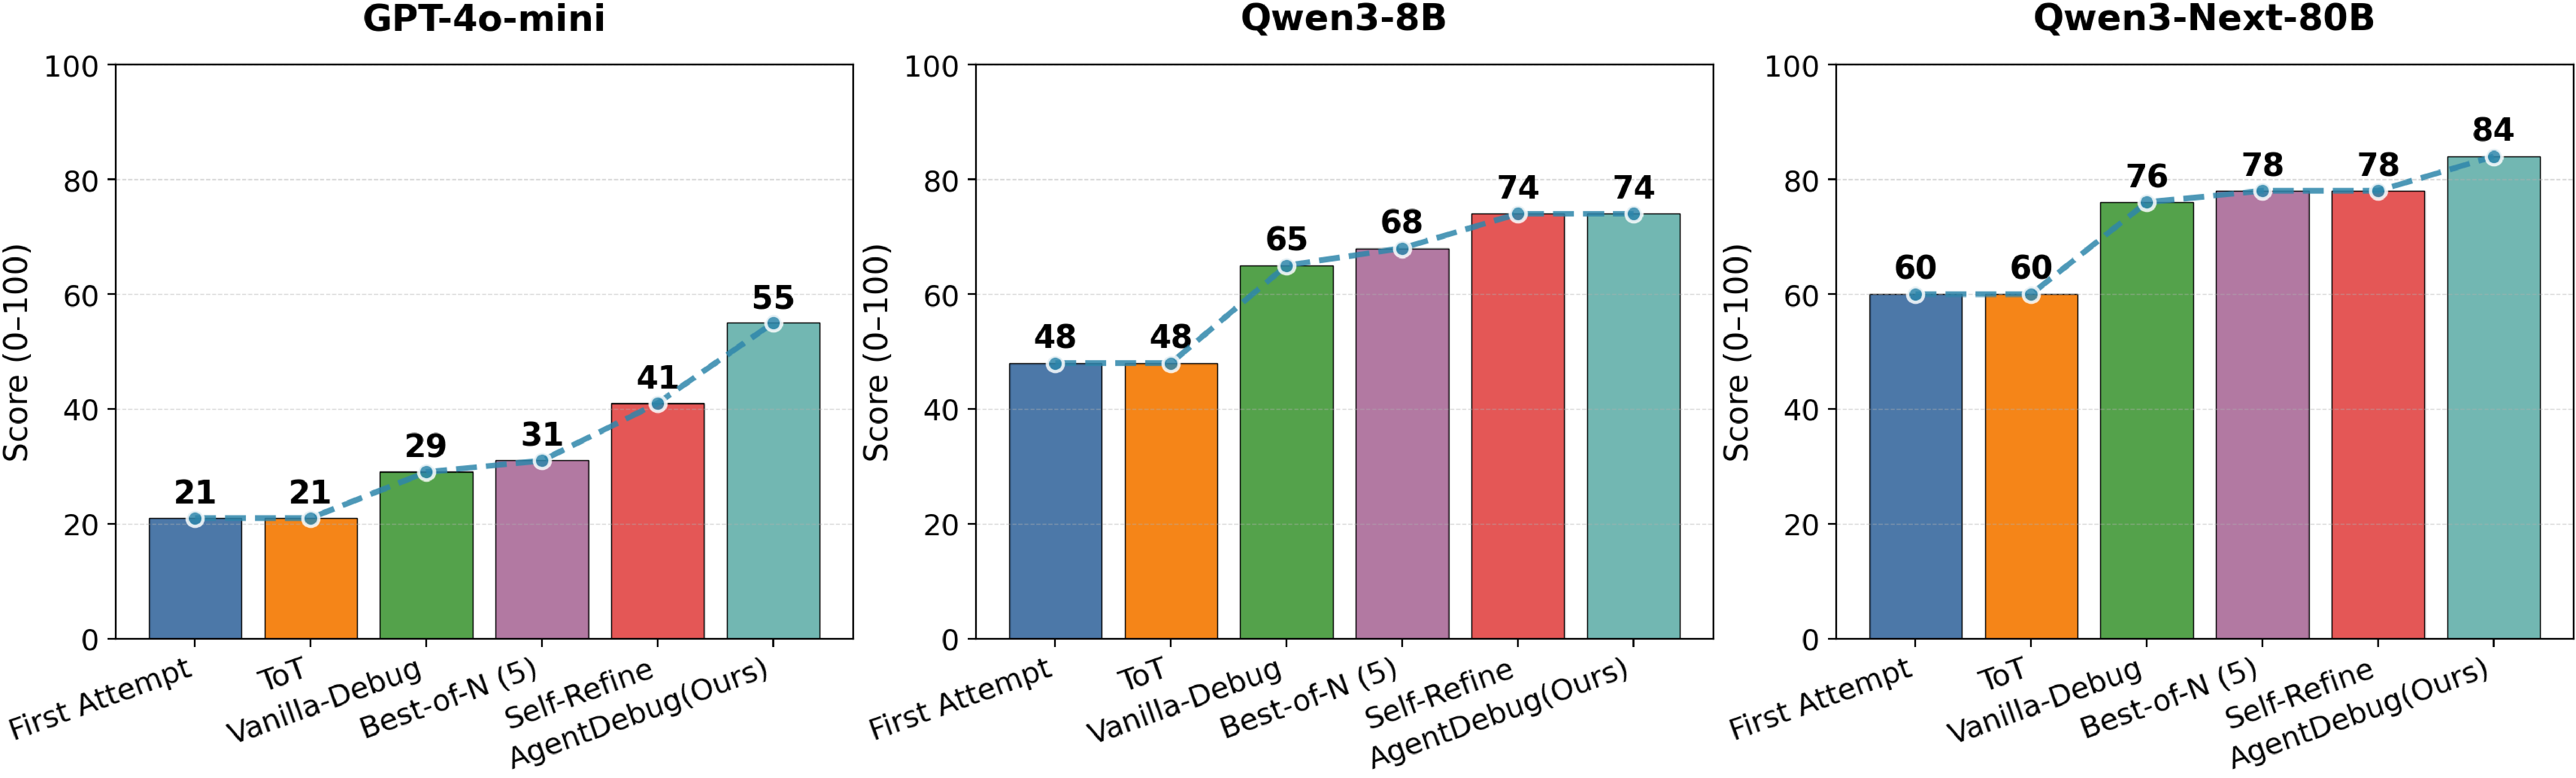
\includegraphics[width=1\linewidth]{iclr2026/figures/agent_tts_alfworld_comparison_tight.pdf}
    \caption{Downstream debugging performance on ALFWorld. Results are shown across three backbone models (GPT-4o-mini, Qwen3-8B, Qwen3-Next-80B) and differnt methods. \ModelName{} consistently outperforms strong baselines.}
    \label{fig:experiment_4_2_1}
\end{figure}

\begin{wrapfigure}{r}{0.40\textwidth}
    \vspace{-6pt} % tighten space above (tweak as needed)
    \centering
    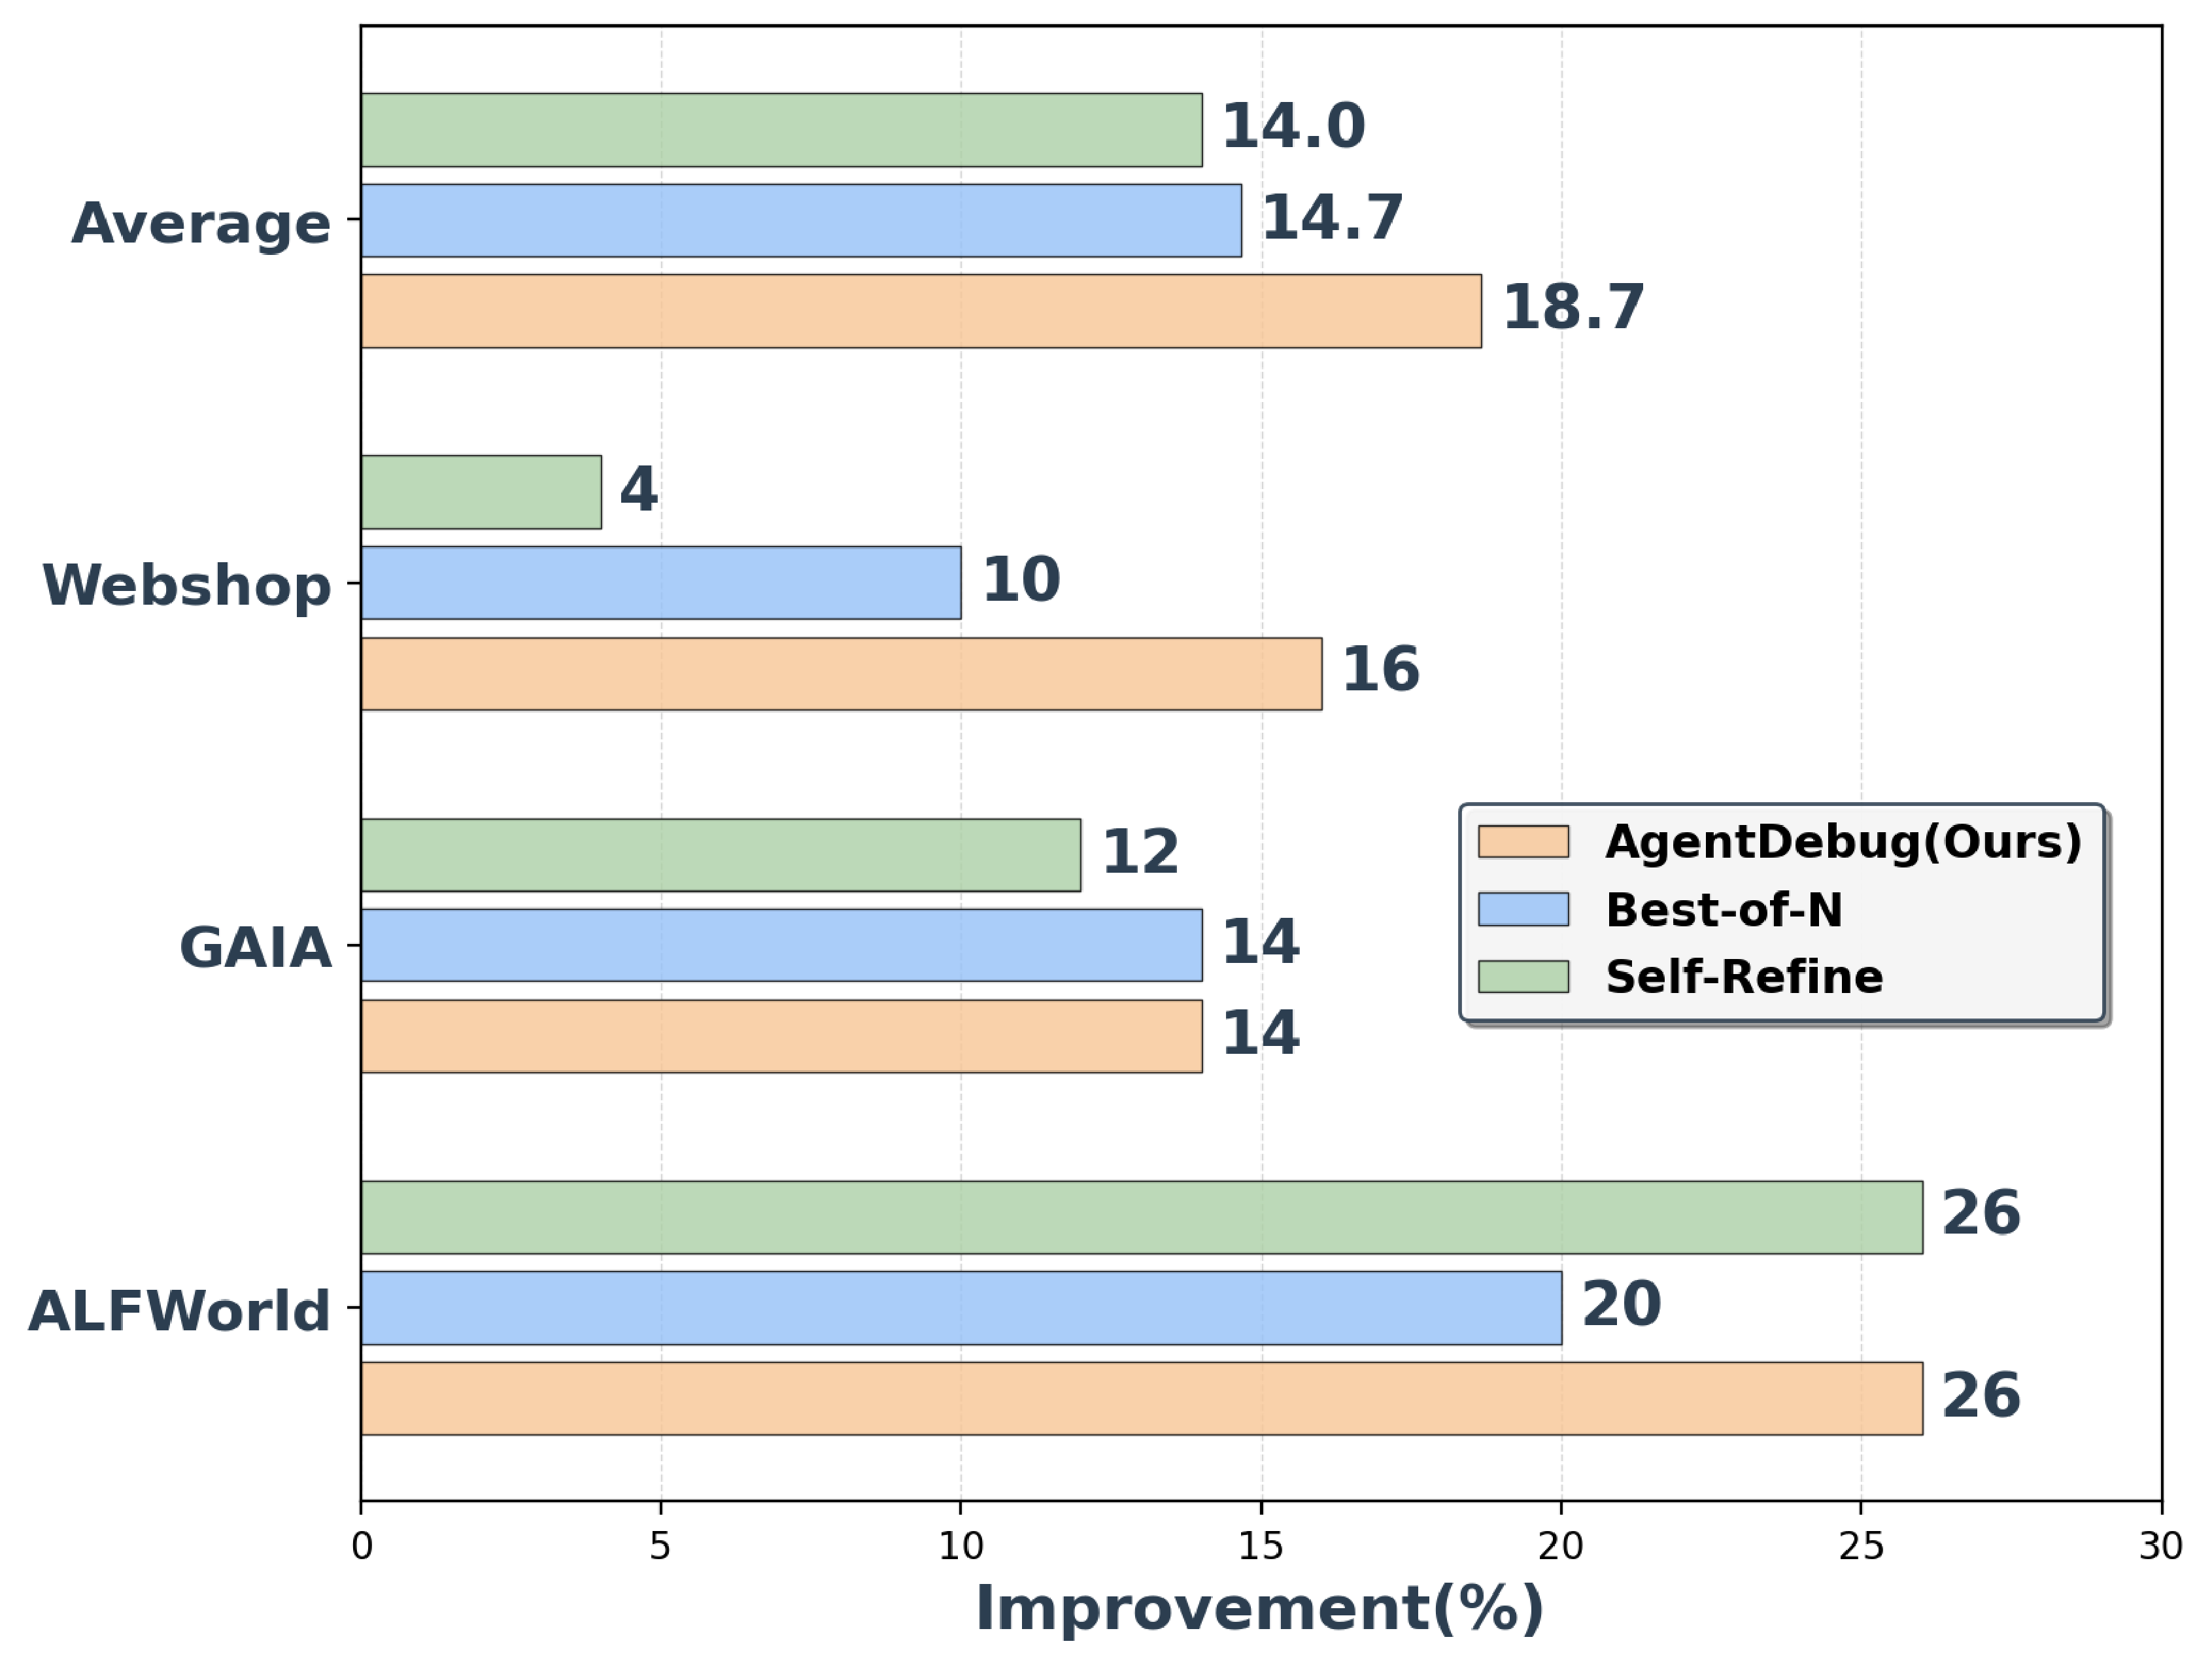
\includegraphics[width=\linewidth]{iclr2026/figures/horizontal_comparison.pdf}
    \caption{Performance improvements comparison.}
    \label{fig:experiment_4_2_2}
    \vspace{-6pt} % tighten space below (tweak as needed)
\end{wrapfigure}


To further assess the generalizability of \ModelName{}, we move beyond ALFWorld and extend our evaluation to two additional benchmarks that stress complementary dimensions of agent reasoning: GAIA, which requires integrating open-domain knowledge and web-based tool use, and WebShop, which evaluates agents in a realistic e-commerce setting with structured constraints and transactional goals. Together, these benchmarks provide a diverse testbed spanning embodied interaction, knowledge-grounded reasoning, and goal-directed web navigation. Given the higher computational demands of these settings, we focus on comparing \ModelName{} against the two strongest baselines from our earlier experiments—Self-Refine and Best-of-$N$—which represent state-of-the-art approaches to iterative refinement and test-time scaling, respectively. The results, shown in Figure~\ref{fig:experiment_4_2_2}, demonstrate that \ModelName{} consistently delivers the largest gains across all three benchmarks. In particular, it achieves improvements of up to 26\% on ALFWorld and strong average performance on GAIA and WebShop, underscoring its robustness across diverse environments and confirming that targeted error detection and correction can outperform broader but less focused strategies such as scaling rollouts or unguided self-revision.


\begin{tcolorbox}[colback=californiagold!5!white, colframe=californiagold!100!black, boxrule=0.5mm, left=0.1mm, right=0.1mm, top=0.1mm, bottom=0.1mm]
\textbf{\textit{Findings}.} \ModelName{} consistently outperforms strong baselines in both error detection and downstream task success. Its ability to precisely localize root-cause failures (50.0\% step accuracy and 42.5\% all-correct accuracy) translates into substantial improvements in task performance, achieving up to 26\% relative gains across ALFWorld, GAIA, and WebShop. 
%These results highlight the effectiveness of principled debugging as a pathway toward more robust LLM agents.
\end{tcolorbox}


% \begin{tcolorbox}[colback=berkeleyblue!5!white, colframe=berkeleyblue!100!black, boxrule=0.5mm, left=0.1mm, right=0.1mm, top=0.1mm, bottom=0.1mm]
% \textbf{Takeaway.} ...
% \end{tcolorbox}

